\clearpage
\onecolumn
\appendix

\section{Game specification and architectural choices}
\label{app:game}

\paragraph{Why this game?}
The fish-delivery race is small enough to expand complete routes, yet contains
sequential consequences: an early road choice changes the stamina and freshness
available later. Branching and rejoining create alternatives without requiring
an open-ended action space. Two porter roles make balance measurable; a visible
moving cloud makes adaptation possible; sampled delays preserve uncertainty.
The map is regenerated between races, so the learned local rule must operate on
unseen combinations of roads rather than memorize a single board. The two
porters do not block, attack, or otherwise change one another's transitions.
Competition is a comparison of deliveries under shared weather, not a model of
strategic opponent interaction.

\begin{figure}[htbp]
\centering
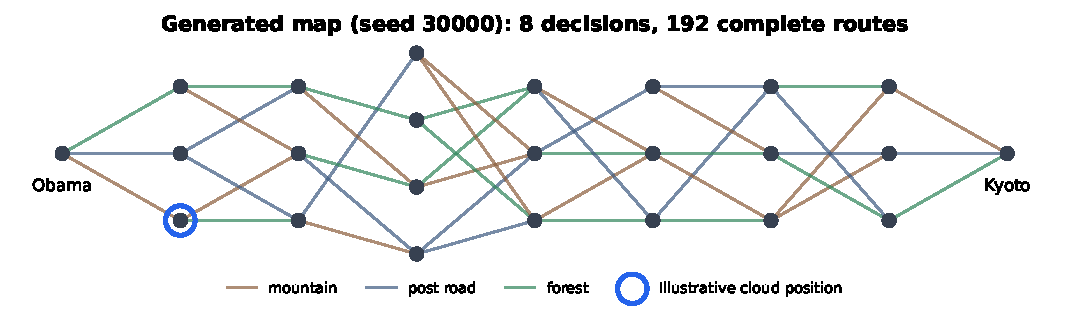
\includegraphics[width=0.94\textwidth]{figures/neural-map.pdf}
\caption{An actual generated test map; roads go from left to right, one layer at
a time. Colors denote terrain, not learned cost. The ring illustrates one legal
initial cloud location, not a measured player trajectory. The graph is shared
by both porters and remains fixed during a race.}
\label{fig:map}
\end{figure}

\paragraph{Map and weather distribution.}
The horizon is uniform on $\{7,8,9,10\}$. The first and last internal layers have
three nodes; the others have three to five. Every destination node receives an
incoming edge; additional links give each source at least two distinct outgoing
roads where possible, with a single common terminal node. Terrain labels are
approximately balanced within each layer transition. Conditional attributes are
sampled independently from the intervals below and rounded to three decimals.
The cloud starts uniformly in the first internal layer, follows a uniformly
sampled outgoing road after each round, and disappears when it reaches the
terminal node. A road is rainy exactly when its destination is the current cloud
node. Exposure is an additional continuous input, not the cloud's transition
probability.

\begin{center}
\begin{tabular}{lcccc}
\toprule
Terrain & Distance & Difficulty & Exposure & Allowed delay event\\
\midrule
Mountain & $U(1.8,3.8)$ & $U(.65,.95)$ & $U(.55,.95)$ & Landslide\\
Forest & $U(2.4,4.5)$ & $U(.30,.70)$ & $U(.15,.55)$ & Fallen tree\\
Post road & $U(3.2,5.5)$ & $U(.05,.35)$ & $U(.25,.65)$ & Cart blockage\\
\bottomrule
\end{tabular}
\end{center}

\paragraph{Information boundary and architecture.}
The local feature vector is
$x=(r_L,r_S,a,f,c,d/5.5,h,e,m_M,m_F,m_P,w)$: role bits, normalized stamina,
freshness, cargo, normalized distance, difficulty, exposure, terrain bits, and
rain. Cargo is fixed at $.75$. All heads have two hidden layers with SiLU
activations and a linear output layer. Their dimensions are:

\begin{center}
\begin{tabular}{llll}
\toprule
Head & Inputs & Layer widths & Output meaning\\
\midrule
Base & $a,f,c,d/5.5,h,e,m_M,m_F,m_P,w$ & $10\to64\to64\to3$ & Time, stamina loss, spoilage rate\\
Role & $h$ & $1\to16\to16\to2$ & Speed and stamina advantages\\
Event & $d/5.5,h,e,m_M,m_F,m_P,w$ & $7\to32\to32\to4$ & Event logits\\
Delay & Same as event head & $7\to32\to32\to3$ & Real-event delays\\
\bottomrule
\end{tabular}
\end{center}

The model has 8,252 trainable parameters. A local MLP is sufficient for these
fixed-size road/state features; a graph network would unnecessarily expose the
mechanic to global position and topology. The \emph{planner}, in contrast,
knows the graph and cloud state. The base and event heads do not see role;
role-dependent behavior enters through explicit difficulty gates. This prevents
direct role-dependent event probabilities, but roles can still encounter
different event frequencies by choosing different roads.

\section{Transition equations and differentiable planning}
\label{app:planning}

\paragraph{A constrained neural rule, not unconstrained rule discovery.}
Writing $\sigma$ for the logistic sigmoid and $(b_T,b_S,b_R)$ for the base-head
outputs, define
\begin{align}
 T_0&=.20+5.80\sigma(b_T), & S_0&=.16\sigma(b_S), & R&=.060\sigma(b_R),\\
 A_T&=.55\sigma(u_T(h)), & A_S&=.55\sigma(u_S(h)),\\
 T&=T_0\exp[-A_T\{r_Sh+r_L(1-h)\}], &
 S&=S_0\exp[-A_Sr_Sh].
\end{align}
Thus light is locally faster on easy roads and strong on hard roads, at otherwise
identical inputs; only strong receives an explicit stamina reduction. These
semantics are architectural constraints, not empirical discoveries. Event
probabilities are a softmax with incompatible terrain events masked to zero;
no event is always allowed. The delay head gives
$\delta_0=0$ and $\delta_k=3\sigma(z_k)$ for each real event. On branch $k$,
\begin{equation}
 (t',a',f')=\bigl(t+T+\delta_k,\ \operatorname{clip}(a-S,0,1),\
 f\exp[-R(T+\delta_k)]\bigr).
\end{equation}
Delay affects time and freshness, not stamina directly. Exhaustion is absorbing
in sampled play, with terminal freshness set to zero. The winner has higher
final freshness; a difference within $10^{-9}$ is a draw. The evaluator stores
physical stamina initialized to 15 and 17, but normalizes before every neural
call and rescales afterward; the normalized dynamics start at one for both roles.

\paragraph{Initialization and inductive bias.}
Output-layer weights start at zero. Biases initialize $T_0=2.4$, $S_0=.065$,
$R=.018$, $A_T=A_S=.20$, compatible-event probability $.20$, and event delay
$.80$. Hidden weights use PyTorch initialization. This starts from a viable,
stochastic rule rather than arbitrary destructive transitions. The DAG, action
space, freshness update, output bounds, terrain masks, and role gates are all
hand-designed. What optimization learns is the local dependence of costs and
events on state, road, and weather within this grammar. There are no observed
next-state labels or teacher-engine regression targets.

\paragraph{Planner and gradient path.}
Let $\bar{s}'_\theta(s,a)$ contain the immediate event-averaged next stamina,
freshness, and elapsed time. In particular,
$\bar f'=\sum_k p_k f\exp[-R(T+\delta_k)]$; the exponential is taken before
averaging. The planner explicitly expands all road and cloud branches but
continues from this \emph{mean event state}, not every sampled event history.
At a terminal state it uses the smooth score
\begin{equation}
 v(a,f)=f\,\sigma((a-.025)/.01)\,\sigma((f-.025)/.01).
\end{equation}
Backward recursion defines uncorrupted action values $Q_0$, reference choices
$\pi_0(a\mid s)=\operatorname{softmax}(35Q_0(s,\cdot))_a$, and
\begin{align}
 Q_\epsilon(s,a)&=\sum_{z'}P(z'\mid z)
 V_\epsilon(\bar{s}'_\theta(s,a),z'),\\
 V_\epsilon(s)&=\sum_a\bigl[(1-\epsilon)\pi_0(a\mid s)+\epsilon U(a\mid s)\bigr]
 Q_\epsilon(s,a).
\end{align}
The same $\pi_0$ is used at every corruption level; it is not reoptimized to
anticipate future mistakes. Gradients pass through neural transitions, event
probabilities, expected states, and soft road choices into the game-level loss.
This is differentiable optimization of a mechanic, not supervised transition
prediction or reinforcement learning of a separate player network.

\paragraph{What hard evaluation changes.}
Hard play recomputes an uncorrupted, full-horizon argmax choice from the actual
current state, then replaces it with a uniformly sampled legal road with
probability $\epsilon$. A replacement can coincide with the reference action:
$\epsilon$ is a replacement probability, not the fraction of objectively wrong
moves. Clouds and events are sampled, and failures stop a porter. The reference
planner still uses mean future event states; ``uncorrupted'' does not mean an
exact solution of the full stochastic game or an optimal win-probability policy.
The train/evaluation differences include soft versus hard decisions, smooth
versus absorbing survival, a sigmoid score-comparison surrogate versus sampled
wins, and expected versus realized future states.

\section{Loss design and numerical specification}
\label{app:loss}

These objectives express a chosen game design. They are not estimates of a
universal definition of quality, nor labels inferred from human enjoyment.
Squared errors give gradients proportional to target mismatch; squared hinge
penalties accept a \emph{range} of viable or stochastic behavior without forcing
all games to one value. Scales below normalize heterogeneous quantities and set
their relative influence. They are fixed design hyperparameters, not the result
of a hyperparameter search.

Let $v_{r,M}(\epsilon)$, $f_{r,M}(\epsilon)$, and $a_{r,M}(\epsilon)$ be planner
outputs, averaged over initial cloud positions. A bar denotes the mean over
sampled maps, and over roles where appropriate. Let $[x]_+=\max(x,0)$,
$d_M=v_{S,M}(0)-v_{L,M}(0)$, and $s(x)=.01\log(1+\exp(x/.01))$.

\paragraph{Viability: avoid both free delivery and unavoidable failure.}
The acceptable terminal score interval is $[.22,.72]$, with at least $.10$
normalized stamina. Using uncorrupted planner outputs,
\begin{align}
 \mathcal L_{\rm viable}
 &=\overline{\left(\frac{[v-.72]_+}{.10}\right)^2
 +\left(\frac{[.22-v]_+}{.10}\right)^2
 +\left(\frac{[.10-a]_+}{.10}\right)^2}\\
 &\quad+.10\,\overline{\sigma((.025-f)/.01)+\sigma((.025-a)/.01)}.
\end{align}
Simply maximizing freshness would permit a trivial mechanic in which every
route delivers perfectly. The upper viability bound avoids that solution;
minimum score and stamina discourage the opposite collapse.

\paragraph{Balance and specialization: fairness without identical roles.}
\begin{align}
 \mathcal L_{\rm balance}&=(\bar d/.025)^2,\\
 \mathcal L_{\rm role}
 &=\left(\frac{\overline{s(d)}-.020}{.015}\right)^2
 +\left(\frac{\overline{s(-d)}-.020}{.015}\right)^2.
\end{align}
Balance concerns the mean \emph{score gap}, not directly the win rate. The role
term asks for advantages in both directions across maps, rather than equal
outcomes on every map. Softplus supplies smooth positive-part estimates, but
$s(0)=.01\log2>0$: a positive diagnostic alone does not prove specialization.
We therefore also report signed-gap fractions and mean absolute gaps. Crucially,
map statistics are pooled \emph{before} squaring; averaging squared singleton
losses would impose a different objective.

\paragraph{Competence response: reward decisions without demanding determinism.}
For $\epsilon_j\in\{0,.25,.50,.75,1\}$, the differentiable focal score is
\begin{equation}
 \hat g_j=\frac12\overline{\sigma\!\left(
 \frac{v_L(\epsilon_j)-v_S(0)}{.025}\right)
 +\sigma\!\left(\frac{v_S(\epsilon_j)-v_L(0)}{.025}\right)},\qquad
 \mathcal L_{\rm skill}=\frac15\sum_j\left(\frac{\hat g_j-y_j}{.10}\right)^2,
\end{equation}
with $y=(.50,.38,.27,.18,.10)$. This deliberately declining target encodes a
preference that better choices matter, while a random focal player retains some
chance against the reference. Its particular shape is not theoretically optimal.
The sigmoid is a differentiable comparison of expected scores, not the expected
win indicator; matching it need not exactly match the hard-play profile.

\paragraph{Weather: a perceptible but bounded challenge.}
Let $\Delta_w=\overline{v_r^{\rm clear}(0)-v_r^{\rm cloud}(0)}$, where the clear
counterfactual disables clouds but retains event randomness. Then
$\mathcal L_{\rm weather}=((\Delta_w-.025)/.015)^2$.
This prevents the network from simply ignoring the visible cloud. The target is
an absolute score reduction, not a relative percentage change.

\paragraph{Luck and semantic regularization: close alternative shortcuts.}
On 96 fixed, deterministic local feature probes, let $\rho=\overline{1-p_0}$ and
$V=\overline{\sum_kp_k\delta_k^2-(\sum_kp_k\delta_k)^2}$. We use
\begin{equation}
 \mathcal L_{\rm luck}=
 \left(\frac{[.12-\rho]_+}{.10}\right)^2+
 \left(\frac{[\rho-.35]_+}{.10}\right)^2+
 \left(\frac{[.04-V]_+}{.10}\right)^2+
 \left(\frac{[V-.80]_+}{.50}\right)^2.
\end{equation}
Both frequency and variance matter: frequent zero-delay events would otherwise
satisfy an event-rate constraint without consequential randomness. These are
probe-distribution quantities, not policy-weighted traversal frequencies.

Counterfactual probes increase normalized distance or difficulty by $.12$,
switch rain off/on, or compare roles at difficulty $.85$ and $.15$. One-sided
ReLU penalties discourage reduced travel/stamina cost on longer or harder roads,
reduced expected travel time or spoilage rate under rain, and reversed role
advantages. The sum is weighted by $.25$. In addition, $10^{-5}$ times the mean
of parameter-tensor mean squares is added; AdamW separately uses weight decay
$10^{-5}$. Probe constraints are soft and finite, not global monotonicity proofs.

\section{Experimental protocol, complete results, and interpretation}
\label{app:results}

\paragraph{A bounded experiment.}
All four nested variants use optimizer seeds $0,1,2$, the same 64 training maps
(seeds $0$--$63$), 16 validation maps ($10000$--$10015$), and 100 test maps
($30000$--$30099$). Training uses AdamW at $.003$, batches of four maps sampled
without replacement within each update, gradient-norm clipping at 5, at most
120 updates, validation every ten updates, and patience six validation checks.
Validation evaluates the pooled objective on the whole validation set. Each
seed's checkpoint minimizes its own variant's validation loss; no test metric
selects checkpoints. All variants are trained from initialization, not continued
from the preceding variant. Different objectives have different numerical
scales, so their raw total losses are not directly comparable.

All reported figures and tables use this matched experiment. The test seed
range is disjoint from the $20000$--$20099$ range used in preliminary experiments;
those earlier results are not mixed into the reported measurements. No further
hyperparameter search was performed for this submission.

Execution was recovered at completed-seed boundaries after a wall-clock limit
and a final-seed GPU-memory failure. The last seed uses per-plan activation
checkpointing, verified against ordinary backpropagation for loss and gradient
agreement, and runs in tmux. This changes the memory/computation trade-off, not
the objective or batch size; incomplete attempts are excluded from per-run times.

\begin{table}[htbp]
\centering
\caption{Matched held-out ablation. Values are means $\pm$ population SD over
three trained seeds, each evaluated on the same 100 maps. All entries are
fractions or normalized scores, not percentages. Base includes viability,
luck, and regularization; later stages add balance, role specialization, and
jointly skill plus weather.}
\label{tab:ablation}
\small
\begin{tabular}{lrrrrr}
\toprule
Variant & Light wins & Freshness & Event rate & Leverage & Tolerance\\
\midrule
Base & $0.667\pm0.031$ & $0.523\pm0.054$ & $0.258\pm0.011$ & $0.432\pm0.027$ & $0.390\pm0.016$\\
+Balance & $0.470\pm0.022$ & $0.644\pm0.023$ & $0.233\pm0.014$ & $0.247\pm0.023$ & $0.478\pm0.024$\\
+Role & $0.500\pm0.008$ & $0.434\pm0.016$ & $0.182\pm0.028$ & $0.493\pm0.006$ & $0.293\pm0.026$\\
Full & $0.560\pm0.029$ & $0.514\pm0.039$ & $0.172\pm0.008$ & $0.475\pm0.004$ & $0.354\pm0.011$\\
\bottomrule
\end{tabular}

\end{table}

\paragraph{What the estimators measure.}
Equal-competence races corrupt both porters at $\epsilon=.2$; reference races
corrupt neither. For every corruption-profile point, one focal role is degraded
and the other remains uncorrupted; both focal assignments are averaged. Score
is 1 for a focal win, $1/2$ for a draw, and 0 for a loss. At $\epsilon=0$, the
two assignments reproduce the same match with complementary focal scores;
$g(0)=.5$ follows by construction and is \emph{not} evidence of role balance.
We instead measure balance through the separate light/strong win rates.

The evaluator uses one seeded realization per map and competence condition,
with cloud, event, and decision random streams shared across model seeds and
variants. Profile streams are reused across corruption levels. Reusing seeds
improves comparability but does not turn the model seeds into independent sets
of maps. Error bars are descriptive across-model SD, not confidence intervals
or significance tests. Mean freshness, failure rates, and event frequencies
refer specifically to the equal-competence races; zero failures there is not a
guarantee about all possible policies or trajectories.

\paragraph{Leverage is not tolerance.}
The CGQ-inspired endpoint summary is $L=g(0)-g(1)$. When $L>0$, normalized
retention is $r(\epsilon)=(g(\epsilon)-g(1))/L$ and tolerance is
$T=\int_0^1r(\epsilon)d\epsilon$, estimated by the trapezoidal rule on the five
reported points. A large leverage means this execution-competence axis affects
outcomes; it does not imply forgiving gameplay. A low tolerance indicates that
much of the advantage is lost early under this particular intervention. These
are policy- and context-dependent signatures, not intrinsic human skill ratings.

\begin{figure}[htbp]
\centering
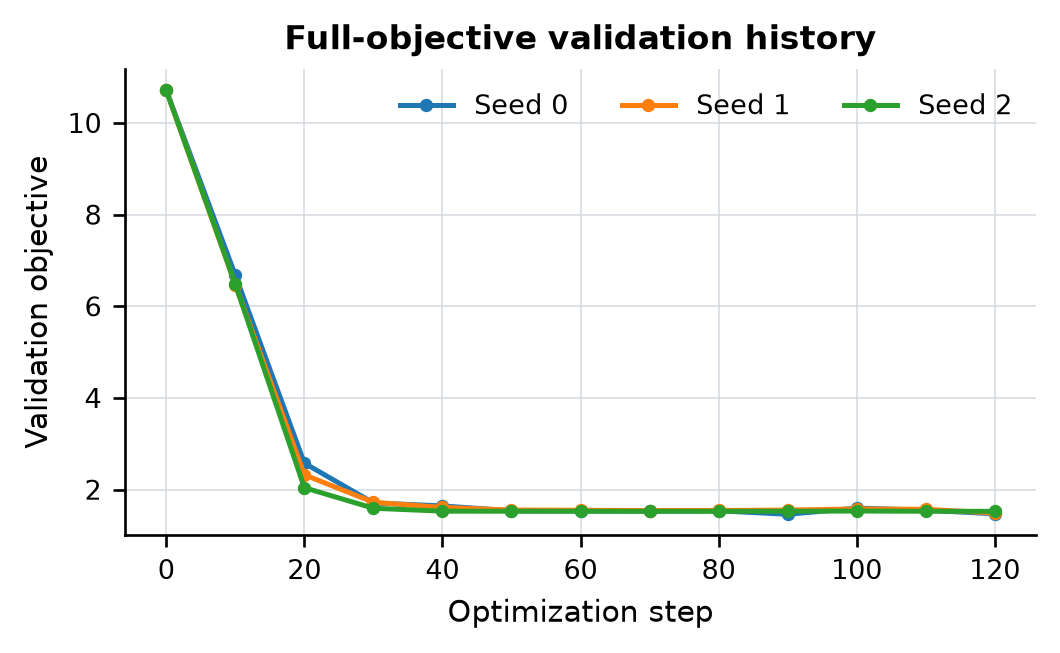
\includegraphics[width=.48\textwidth]{figures/neural-training.png}\hfill
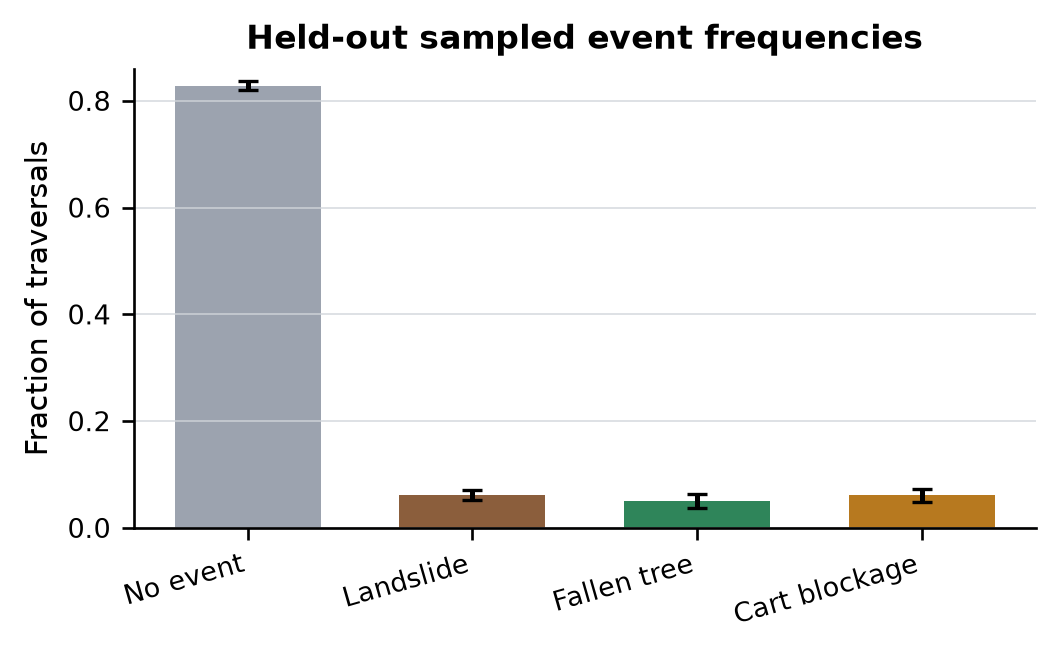
\includegraphics[width=.48\textwidth]{figures/neural-event-frequencies.png}
\caption{Left: full-objective validation histories used for checkpoint
selection. Right: sampled event frequencies in held-out equal-competence races;
error bars are population SD across model seeds. Terrain frequencies and route
choices affect these counts, so they need not equal the local probe rate.}
\label{fig:training-events}
\end{figure}

\section{Per-seed evidence and remaining limitations}
\label{app:limits}

\begin{table}[htbp]
\centering
\caption{Every executed final run. Seconds include training, validation, and
hard evaluation, not just optimizer time. Failure fractions are measured in
equal-competence races. The distributed full-model checkpoint is seed
\SelectedSeed{}, selected by validation loss rather than test performance.}
\small
\begin{tabular}{lrrrrrr}
\toprule
Variant & Seed & Best step & Validation loss & Light wins & Failures & Seconds\\
\midrule
Base & 0 & 60 & 0.0000 & 0.650 & 0.000 & 112.1\\
Base & 1 & 30 & 0.0000 & 0.710 & 0.000 & 102.5\\
Base & 2 & 30 & 0.0000 & 0.640 & 0.000 & 103.1\\
+Balance & 0 & 70 & 0.0000 & 0.480 & 0.000 & 110.4\\
+Balance & 1 & 120 & 0.0000 & 0.490 & 0.000 & 111.4\\
+Balance & 2 & 110 & 0.0000 & 0.440 & 0.000 & 110.3\\
+Role & 0 & 90 & 0.7253 & 0.490 & 0.000 & 110.6\\
+Role & 1 & 120 & 0.8318 & 0.500 & 0.000 & 110.9\\
+Role & 2 & 120 & 0.6844 & 0.510 & 0.000 & 110.4\\
Full & 0 & 90 & 1.4610 & 0.600 & 0.000 & 135.8\\
Full & 1 & 120 & 1.4877 & 0.550 & 0.000 & 133.4\\
Full & 2 & 120 & 1.5246 & 0.530 & 0.000 & 160.9\\
\bottomrule
\end{tabular}

\end{table}

\begin{table}[htbp]
\centering
\caption{Full-model diagnostics at the selected checkpoints. Role and weather
quantities are validation-surrogate measurements on 16 maps; the difficulty
penalty is computed on the fixed semantic probe set. They are not additional
held-out hard-play measurements.}
\small
\begin{tabular}{lrrr}
\toprule
Quantity & Seed 0 & Seed 1 & Seed 2\\
\midrule
Mean role gap (strong minus light) & -0.0031 & 0.0014 & -0.0014\\
Mean absolute role gap & 0.0065 & 0.0059 & 0.0027\\
Strong-favored map fraction & 0.2500 & 0.5000 & 0.2500\\
Light-favored map fraction & 0.7500 & 0.5000 & 0.7500\\
Cloud cost & 0.0288 & 0.0292 & 0.0267\\
Difficulty penalty & 0.0552 & 0.0607 & 0.0557\\
\bottomrule
\end{tabular}

\end{table}

\begin{figure}[htbp]
\centering
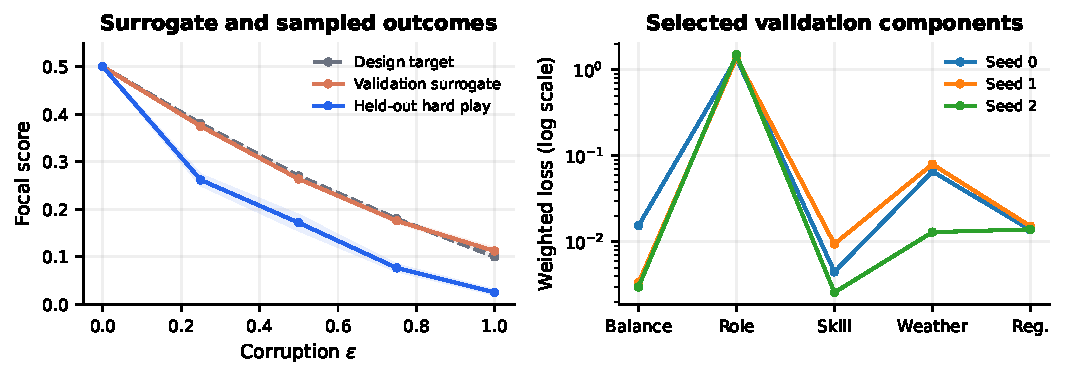
\includegraphics[width=.96\textwidth]{figures/neural-surrogate-diagnostics.pdf}
\caption{Left: the design target, selected validation-surrogate profiles, and
held-out hard profiles; shading is across-seed population SD. Different map
sets and multiple estimator differences contribute to the gap, so this is not
an isolated measurement of event-averaging bias. Right: remaining weighted loss
components at the selected full checkpoints. Components are nonnegative;
viability and luck can be inactive inside their acceptable ranges.}
\label{fig:surrogate}
\end{figure}

\paragraph{Interpreting the residuals.}
Figure~\ref{fig:surrogate} shows that the validation surrogate closely follows
the chosen competence target while sampled play penalizes corruption more
strongly. The full-model tolerance is $\FullTolerance$: high leverage should
not be mistaken for gentle degradation. Weather cost is near its target, but
the role-specialization term remains a major residual. Its softplus advantages
remain below $.020$, and the small absolute score gaps do not establish robust
map-dependent specialization. Difficulty penalties also remain positive: soft
local regularization has not guaranteed monotone behavior. These are observable
limits of this short optimization, not properties the report assumes away.

\paragraph{What this establishes, and what it does not.}
The experiment tests whether a constrained local neural rule can be optimized
through differentiable game-level objectives and then used in sampled play on
held-out maps. It does not show that every loss target is achieved, that
specialization is robust to a different map distribution, or that the resulting
game is enjoyable for humans. Only three optimizer seeds, a short training
budget, and one stochastic realization per map-condition are used. The nested
ablation measures incremental changes in this order; skill and weather enter
together, so their individual causal effects are not identified. The absence
of a transition teacher does not remove human design choices from the grammar,
initialization, or loss. Useful next steps are matched stochastic estimators,
more weather/event repetitions, a factorial loss ablation, held-out role and
cloud counterfactuals, and human playtesting.

\paragraph{Reproducibility.}
The repository contains the selected state dictionary in
\texttt{results/selected\_model.json}, all final protocol/history/metric records
in \texttt{results/neural-evaluated.json}, and the figure/table builder
\texttt{mackerel\_road.experiments.submission}. The reporting path uses stored
measurements and requires no GPU or PyTorch. The full training command and
verification instructions are in \texttt{README.md} and
\texttt{report/README.md}. Raw run payloads retain all seed checkpoints locally;
only the selected checkpoint is included in the submission repository.
